\documentclass[a4paper, 12pt]{article}

\usepackage{cmap}
\usepackage{mathtext} 
\usepackage[T2A]{fontenc}
\usepackage[utf8]{inputenc}
\usepackage[english,russian]{babel}	

\usepackage{amsfonts,amssymb,amsthm,mathtools}
\usepackage{amsmath}
\usepackage{icomma} 

\usepackage{graphicx} 
\graphicspath{{Picturies/}}
\usepackage{wrapfig}

\usepackage{array,tabularx,tabulary,booktabs}
\usepackage{longtable}
\usepackage{multirow}

\usepackage{caption}
\captionsetup{labelsep=period}

\renewcommand{\phi}{\varphi}
\newcommand{\eps}{\varepsilon}
\renewcommand{\AA}{\ensuremath{\mathring{A}}}
\newcommand{\parag}[1]{\paragraph*{#1:}}

\newcounter{Points}
\setcounter{Points}{1}
\newcommand{\point}{\arabic{Points}. \addtocounter{Points}{1}}

\author{Вязовцев Андрей, Б01-009}
\date{16.11.22}
\title{Лабораторная работа 5.10.1. Электронный парамагнитный резонанс.}

\begin {document}

\maketitle

\parag {Цель работы} исследовать электронный парамагнитный резонанс (ЭПР) в молекуле дифенилпикрилгидразила (ДФПГ), определить $g$-фактор электрона, измерить ширина линий ЭПР.

% \parag {В работе используются}

% Спасибо блек саморезу за возможность переебать теорию и текст.

\parag {Теоретическая справка} ~\\

Энергетический уровень электрона в присутствии магнитного поля с индукцией $B$ расщепляется на подуровня, расстояние между которыми равно 
\begin{equation}
    \label{eq:dE}
    \Delta E = E_2 - E_1 = 2\mu B.
\end{equation}
Здесь $\mu$ -- абсолютная величина проекции магнитного момента на направление поля.

Между этими двумя уровнями возможны переходы. Эти переходы могут возбуждаться внешним высокочастотным электромагнитным полем, если оно имеет нужную частоту и нужное направление.

Резонансное значение частоты определяется из очевидной формулы:
\begin{equation}
    \label{eq:resonans_omega}
    \hbar \omega_0 = \Delta E.
\end{equation}

При переходе с нижнего на верхний уровень энергии электрон поглощает квант электромагнитной энергии, а при обратном переходе такой же квант излучается. Возбуждение электронных резонансных переходов электромагнитным полем, имеющим частоту, определяемую формулой~(\ref{eq:resonans_omega}), носит название электронного парамагнитного резонанса (ЭПР).

В настоящей работе необходимо получить сигнал ЭПР на кристаллическом дифенилпикрилгидразиле (ДФПГ) и определить значение $g$-фактора для электрона. Как известно, связь между магнитным моментом $\mu$ электрона и его механическим моментом $\mathbf{M}$ выражается через гиромагнитное отношение $\gamma$ с помощью формулы

\begin{equation}
    \label{eq:gyromagnit}
    \mu = \gamma M.
\end{equation}

А магнитный момент частицы, измеренный в магнитонах Бора, а механический - в $\hbar$, то их связь можно записать через $g$-фактор:

\begin{equation}
    \label{eq:def_g}
    \frac{\mu}{\mu_Б} = \frac{M}{\hbar} 
\end{equation}

Используя соотношения (\ref{eq:dE})-(\ref{eq:def_g}), нетрудно получить выражение для $g$-фактора через определяемые экспериментально величины:

\begin{equation}
    \label{eq:g_is}
    \tag{$\star$}
    g = \frac{\hbar \omega_0}{\mu_Б B}.
\end{equation}

\parag {Экспериментальная установка} ~

В работе исследуется ЭПР в дифенилпикрилгидразиле,
сокращённо обозначаемом ДФПГ (DPPH в
англоязычной литературе). Химическая формула этого
соединения $C_{18} H_{12} N_5 O_6$, молярная масса 394 г/моль.

\begin{figure}[!h]
    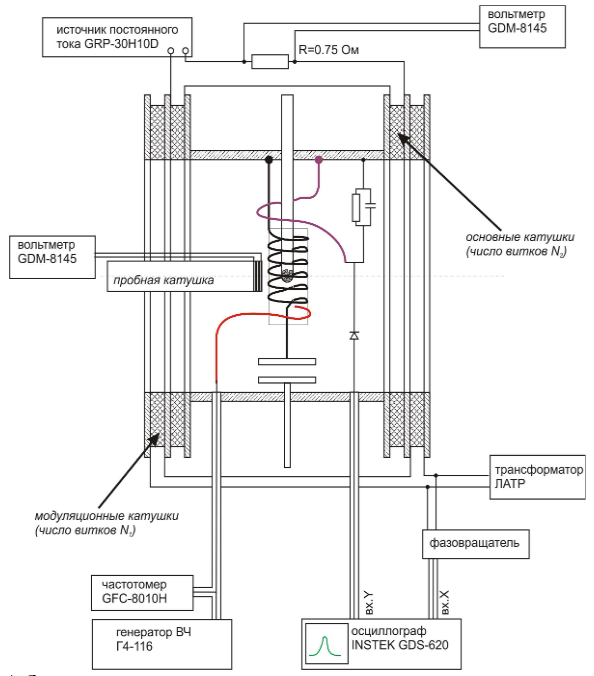
\includegraphics[scale = 0.5]{Workplace}
    \centering
    \caption{Схема установки}
    \label{img:work}
\end{figure}

\newpage

\parag {Ход работы} ~\\

\point Перед началом работы запишем параметры установки (см. табл. \ref{tab:kat}).

\begin{table}[!h]
    \centering
    \begin{tabular}{|c|c|c|}
        \hline
        Катушка & $N$ & $D$, мм \\ \hline
        Основная      & 1500 & $230  \pm 10$  \\ \hline
        Модуляционная & 4500 & $290  \pm 10$  \\ \hline
        Пробная       & 45   & $14.5 \pm 0.1$ \\ \hline
    \end{tabular}
    \caption {Парамерты катушки}
    \label{tab:kat}
\end{table}

\point Включим установку. Настроим генератор на частоту колебательного контура. Получаем резонансу частоту:

\[
    f_0 = 125 \pm 1 ~ МГц
\]

Подберем величину постоянного магнитного поля в катушках так, чтобы наблюдался сигнал резонанского поглощения. Для этого подадим на катушки достаточное напряжение.

Для более точной настройки и определения ширины линии резонасного поглощения будем наблюдать сигнал в $XY$-режиме. Запишем значение напряжения на резисторе в цепи основных катушек:
		
\begin{equation*}
    U_0 = (126 \pm 1) ~мВ
\end{equation*}

\point Определим ширину линии ЭПР (полуширина на на полувысоте линии резонасного поглощения):

\begin{equation*}
    \Delta B = \frac{A_{1/2}}{A_{полн}}B_{мод},
\end{equation*}

где $A_{полн}$ -- полный размах модулирующего поля, $A_{1/2}$ -- ширина кривой на полувысоте, $B_{мод}$ -- амплитуда модулирующего поля.

\begin{equation*}
    \begin{gathered}
        A_{полн} = (10 \pm 0.2) ~дел, ~ A_{1/2} = (3.2 \pm 0.2) ~дел \\
        B_{мод} = \sqrt{2} \frac{2\eps}{\pi^2d^2N\nu} = (0.39 \pm 0.02) ~мТл,
    \end{gathered}
\end{equation*}

где $\eps$ -- ЭДС индукции при внесении пробной катушки, $N$ -- число витков катушки, $d$ -- диаметр катушки, $\nu$ -- частота модулирующего напряжения (50 Гц).

Имеем:

\[
    \Delta B = (0.12 \pm 0.01) ~мТл
\]

\point Калибровка основной катушки.

Определим связь между падением напряжения на резисторе в цепи основных катушек и магнитным полем в центре магнита. Поле в центре будем измерять, поднося пробную катушку к основным с двух сторон - спереди и сзади. В качестве значения поля возьмем среднее этих величин. Результаты занесем в Таблицу \ref{table:field}: 

\begin{table}[h]
\centering
\begin{tabular}{|c|c|c|c|c|c|c|c|c|c|}
    \hline
    $V_R$, мВ              & 126.0 & 20.0 & 40.7 & 60.0 & 80.0 & 100.5 & 120.7 & 140.2 & 160.0 \\ \hline
    $V_{перед}$, мВ & 10.66 & 1.69 & 3.45 & 5.1 & 6.79 & 8.54 & 10.2 & 11.78 & 13.5 \\ \hline
    $V_{зад}$, мВ   & 10.88 & 1.67 & 3.46 & 5.12 & 6.97 & 8.56 & 10.24 & 11.88 & 13.58 \\ \hline
    $V_{сред}$, мВ  & 10.77 & 1.68 & 3.455 & 5.11 & 6.88 & 8.55 & 10.22 & 11.83 & 13.54 \\ \hline
\end{tabular}
\caption{Калибровочные измерения}
\label{table:field}
\end{table}

Методом наименьших квадратов найдем коэффициент пропорциональности между напряжением на основных катушках и напряжением на пробной катушке:
\begin{equation*}
    k = 0.0846 \pm 0.0004
\end{equation*}

Рассчитав поле, создаваемое основными катушками,

\begin{equation*}
    B_0 = \frac{4 k U_0}{2\pi\nu N \pi d^2} = (4.6 \pm 0.3) ~мТл
\end{equation*}

Найдем $g$-фактор электрона:

\begin{equation*}
    g = \frac{hf_0}{\mu_BB_0} = 1.94 \pm 0.12
\end{equation*}

\parag{Вывод} ~\\

В данной работе был исследован ЭПР в молекуле ДФПГ, определяется $g$-фактор электрона $g = 1.94 \pm 0.12$, а также измерена ширина линий ЭПР $\Delta B = (0.12 \pm 0.01) ~мТл$. 
Измеренный $g$-фактор электрона совпадает с табличным значением для свободного электрона: $g = 2,0$. Это обусловлено тем, что ПР происходит на неспаренных электронах так же, как на свободных.

% \parag {Обработка результатов} ~\\

% \point 

\end {document}
